\documentclass[12pt, a4paper] {article}
\usepackage[T2A]{fontenc}
\usepackage[english, russian] {babel}
\usepackage[usenames,dvipsnames]{xcolor}
\usepackage{fontspec}
\setmainfont{Times New Roman}
\setsansfont{Arial}
\setmonofont{Courier New}
\newfontfamily\cyrillicfont[Script=Cyrillic]{Times New Roman}
\newfontfamily\cyrillicfontsf[Script=Cyrillic]{Arial}
\newfontfamily\cyrillicfonttt[Script=Cyrillic]{Courier New}
\usepackage{minted,a4wide,longtable,amsmath,amsfonts,graphicx,tikz}
\usepackage{indentfirst,verbatim}

\begin{document}
\thispagestyle{empty}
\begin{center}
  {\large
    Университет ИТМО \\
    Кафедра Вычислительной техники \\
  }
\end{center}
\vspace{\stretch{2}}
\begin{center}
  Курсовая работа по дисциплине\\
  {\large
    ``Информационно-управляющие системы''\\
    ``Разработка контроллера кодового замка''\\
  }
\end{center}
\vspace{\stretch{6}}
\begin{flushright}
  Работу выполнили студенты группы P3415\\
  {\it Фомин Евгений\\
    Фролов Сергей \\
    Кобзарев Дмитрий \\
    Хайруллин Вадим \\
    Халанский Дмитрий \\
  }
\end{flushright}
\vspace{\stretch{4}}
\begin{center}
  2016 
\end{center}
\newpage

\section{Разработка технического задания}
\subsection{Предмет разработки}
Информационно-управляющая система для кодового замка.
\subsection{Представленные на рынке решения}
Контроллер для кодового замка представляет собой устройство, которое:
\begin{enumerate}
  \item Обрабатывает сигналы, поступающие с панели управления
  \item Управляет закрытием/открытием замка исходя из правильности введенного кода
  \item Сбрасывает ввод кода при превышении лимита времени между нажатиями
  \item Обеспечивает индикацию правильности введеного кода
  \item Производит логирование
\end{enumerate}
\subsubsection*{Микроконтроллеры STM32F1}
Серия STM32F1 представлена микроконтроллерами на 32-битном
процессорном ядре Cortex-M3, выпускаемая ST Microelectronics. В отличие от
мк других серий, обладают меньшим набором периферии, меньшей
производительностью, но и невысокой стоимостью.
Отличительные черты контроллеров:
\begin{enumerate}
  \item разрядность 32 бит;
  \item распространненая архитектура ARM;
  \item поддержка основных интерфейсов обмена данными: SPI, I2C, UART, USB;
  \item соотношение цены и характеристик;
  \item большое число линий ввода-вывода и прерываний;
  \item управление частотой для реализации режима пониженного энергопотребления;
  \item малые габаритные размеры корпуса;
  \item наличие втроеной flash-памяти для программ.
\end{enumerate}
Цена за штуку варьируется от 100 до 400 руб.
\subsubsection*{Микроконтроллеры AVR}
Микроконтроллеры AVR представлены моделями ATmega8, ATtiny13, 
ATtiny2313. Производятся компанией ATMEL. Отличительные особенности 
контроллеров:
tinyAVR:
\begin{enumerate}
  \item Флеш-память до 16 Кб, SRAM до 512 б, EEPROM до 512 б;
  \item Число линий ввода-вывода 4-18;
  \item Ограниченный набор переферийных утройств.
\end{enumerate}

megaAVR:
\begin{enumerate}
  \item Флеш-память до 256 Кб, SRAM до 16 Кб, EEPROM до 4 Кб;
  \item Число линий ввода-вывода 23-86;
  \item Аппаратный умножитель;
  \item Расширенная система команд и переферийных устройств.
\end{enumerate}
Цена за штуку составляет от 150 до 170 руб.

\subsection{Описание разрабатываемой системы}
\subsubsection*{Функциональность разрабатываемой ИУС}
\begin{enumerate}
  \item Управление замком посредством ввода кода
  \item Возможность изменить код открытия замка
  \item Просмотр лога ввода кодов
  \item Индикация успешного/неудачного ввода кода
\end{enumerate}
\subsubsection*{Ограничения на применение ИУС}
ИУС разрабатывается для кодовых замков и область ее применения
ограничивается только ими.
\subsubsection*{Ограничения на реализацию ИУС}
Аппаратное обеспечение:
\begin{enumerate}
  \item Микроконтроллер STM32F103C8T6
  \item ЖКИ J204A на базе HD44780 с I2C модулем 
  \item Часы реального времени DS3231
  \item Безымянная матричная клавиатура
  \item EEPROM AT24C04A
\end{enumerate}
Программные средства:
\begin{enumerate}
  \item Компилятор arm-none-eabi-gcc
  \item ST-Link/v2
\end{enumerate}

\subsection{Режимы работы}
\begin{itemize}
  \item Режим ожидания/Пользовательский режим
  \item Режим обслуживания
\end{itemize}
\begin{figure}[h!]
  \centering
  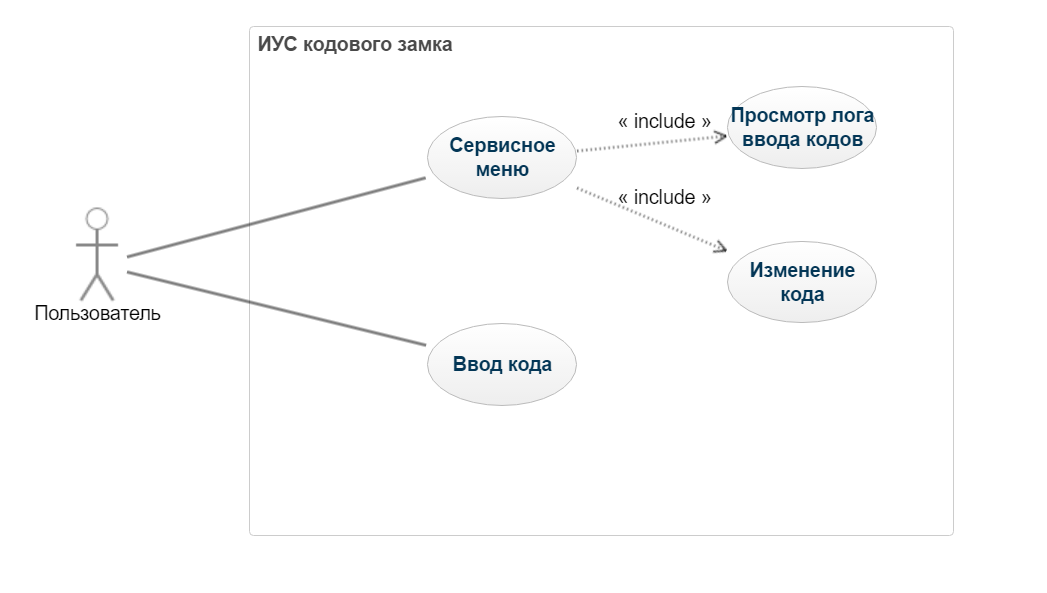
\includegraphics[width=0.8\textwidth]{usecase}
  \caption{Диаграмма прецедентов использования}
\end{figure}
\subsubsection*{Пользовательский режим}
В пользовательском режиме работы система большую часть
времени ожидает ввода кода пользователем. Рабочий процесс
начинается с момента ввода пользователем первой цифры кода:
ИУС ожидает ввода оставшихся трех цифр и принимает решение,
открыть ли замок или нет. При правильном вводе происходит
индикация светодиодом (открытие двери) и сообщение ``OK'', иначе сообщение о
неправильном вводе. В обоих
случаях происходит запись в лог. Третий возможный сценарий
при первом и последующих нажатий до четырех подразумевает
отмену ввода при превышении времени интервала между нажатиями.
В этом случае происходит возврат в
режим ожидания и запись в лог.
\subsubsection*{Режим обслуживания}
В режиме обслуживания система позволяет выполнять две операции:
изменение кода замка и просмотр логов. Запись в журнале
включает в себя информацию о дате и времени события и его исход
(успешный ввод, неверный код или отмена).

\subsection{Перспективные возможности ИУС}
\begin{itemize}
  \item Возможность сохранения нескольких кодов
  \item Подача звуковых сигналов при нажатии клавиш
  \item Подача звуковых сигналов при открытии/закрытии замка
  \item Удаление отдельно взятых записей лога
\end{itemize}

\section{Разработка архитектуры ИУС}
\subsection{Переферийные устройства}
В работе ИУС задействованы следующие устройства:
\begin{itemize}
  \item Часы реального времени требуются для информации в логе
  \item Клавиатура -- для ввода кода, настройки и просмотра логов
  \item Энергонезависимая память -- хранение логов и кода
  \item Панель светодиодов -- индикация после ввода кода
  \item ЖКИ -- просмотр логов, вывод количества введенных цифр
\end{itemize}

\subsection{Особенности разрабатываемой ИУС с точки зрения пользователя}
Назначение ИУС и интерфейс взаимодействия минимизированы, что не требует
обучения для пользования системой. Для того, чтобы начать ввод кода не
требуется никаких дополнительных действий -- система перейдет из режима ожидания
по первому нажатию, ожидая следующей цифры кода. Для отмены так же не требуется
никаких действий со стороны пользователя -- отмена происходит спустя небольшой
промежуток времени. Количество введенных символов отображается на экране.
Отдельной группой пользователей являются люди, имеющие доступ к сервисному меню.
Возможности ИУС для них шире, однако количество усложнений сведено к минимуму.
\subsection{Особенности разрабатываемой ИУС с точки зрения разработчика}
Разработка ИУС ведется на языке C с использованием драйверов для выбранной
переферии. Так как логика работы системы достаточно последовательна, ее можно
представить в коде программы как конечный автомат с некоторым количеством
состояний. Переходы между ними во многом зависят от времени, поэтому применяются
таймеры для отчета времени между нажатиями, время открытия двери. Не очень
большую по своему объему главную логику можно обособить в один модуль.

\begin{figure}[h!]
  \centering
  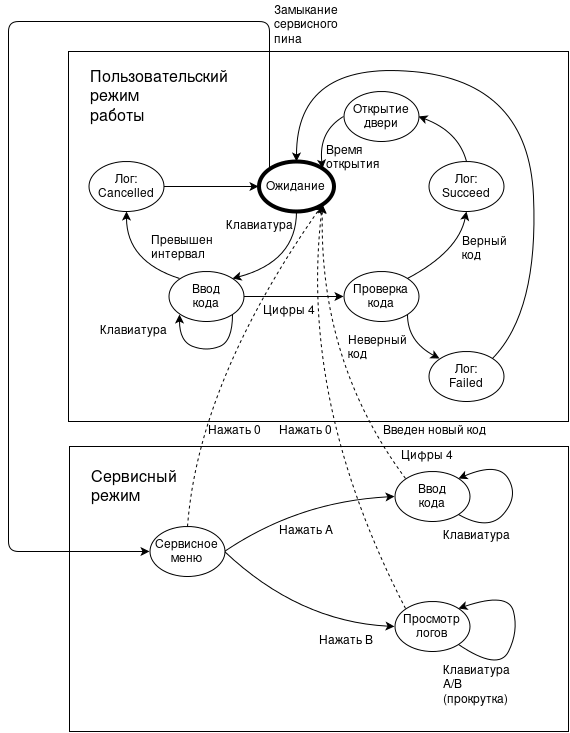
\includegraphics[width=0.8\textwidth]{diag}
  \caption{Основная логика ИУС}
\end{figure}

Таким образом, программное обеспечение разбито на модули:
\begin{itemize}
  \item Драйвер часов реального времени
  \item Драйвер клавиатуры
  \item Драйвер светодиодной панели
  \item Драйвер ЖКИ
  \item Драйвер энергонезависимой памяти
  \item Модуль основной логики ИУС
\end{itemize}

\subsubsection*{Возможности расширения ИУС}
\begin{description}
\item[Возможность сохранения нескольких кодов] Изменения затронут модуль
  основной логики: реализовать добавление/удаление кодов, просмотр текущих
  кодов, логирование с конкретизацией введенного кода
\item[Подача звуковых сигналов] Написание драйвера звукоизлучателя
\item[Удаление записей логов] Изменить структуру хранения записей
  
\end{description}
\newpage

\section{Исходный код основного модуля}
\inputminted{c++}{main.c}


\end{document}